\documentclass[a4paper,11pt,twoside]{article}
%\documentclass[a4paper,11pt,twoside,se]{article}

\usepackage{UmUStudentReport}
\usepackage{verbatim}   % Multi-line comments using \begin{comment}
\usepackage{courier}    % Nicer fonts are used. (not necessary)
\usepackage{pslatex}    % Also nicer fonts. (not necessary)
\usepackage[pdftex]{graphicx}   % allows including pdf figures
\usepackage{listings}
%\usepackage{lmodern}   % Optional fonts. (not necessary)
%\usepackage{tabularx}
%\usepackage{microtype} % Provides some typographic improvements over default settings
%\usepackage{placeins}  % For aligning images with \FloatBarrier
%\usepackage{booktabs}  % For nice-looking tables
%\usepackage{titlesec}  % More granular control of sections.

% DOCUMENT INFO
% =============
\department{Institution för Datavetenskap}
\coursename{Datavetenskapens byggstenar 7.5 p}
\coursecode{DV160HT15}
\title{OU4 Analysis of Complexity}
\author{Lorenz Gerber  ({\tt{dv15lgr@cs.umu.se}})}
\date{2015-12-25}
%\revisiondate{2015-09-15}
\instructor{Lena Kallin Westin / Johan Eliasson}


% DOCUMENT SETTINGS
% =================
\bibliographystyle{plain}
%\bibliographystyle{ieee}
\pagestyle{fancy}
\raggedbottom
\setcounter{secnumdepth}{2}
\setcounter{tocdepth}{2}
%\graphicspath{{images/}}   %Path for images

\usepackage{float}
\floatstyle{ruled}
\newfloat{listing}{thp}{lop}
\floatname{listing}{Listing}


% DEFINES
% =======
%\newcommand{\mycommand}{<latex code>}

% DOCUMENT
% ========
\begin{document}
\lstset{language=C}
\maketitle

\tableofcontents
\newpage

\section{Introduction} 
The aim with this laboration was to apply experimental and asymptotic
complexity analysis of algorithms. 

What is complexity analysis. Experimental, asymptotic. What is big O
notation, what does it mean.
\subsection{The `Big O' notation'}
`Ordo' or `Big O' notation is a mathematical definition on the
complexity of an algorithm. It can be written as shown in 
equation (\ref{eq:ordo})\cite[pp. 245]{janlert2000}.

\subsection{Determining of \textit{Ordo}, $c$ and $n_{0}$}
bla bla bla

\begin{equation} \label{eq:ordo}
f(n) \Rightarrow O(g(n)) \textrm{ if } f(n) \leq c \times g(n)
\textrm{ for } n \geq n_{0} \textrm{ and }
c > 0 \textrm{ and } n_{0} \geq 1
\end{equation}

bla bla bla

\begin{equation} \label{eq:limes}
\lim_{n \to \infty} {f(n) \over g(n)} + 1
\end{equation}



\section{Material and Methods}

\subsection{Experimental Complexity Analysis}
Describe experiment, describe the rules.

\subsection{Asymptotic Complexity Analysis}
Describe what was given and the rules to analyse.
\begin{listing}\label{ls:bubble}
\begin{verbatim}
Algorithm bubbleSort(numElements, list[])
input:  numElements, the number of elements in the list
        list, a list of numbers to be sorted
output: the sorted list

1:  done <- false
2:  n <- 0
3:   while (n < numElements) and (done = false)
4:      done <- true
5:      for m <- (numElements -1) downto n
6:          if list[m] < list[m - 1] then
7:              tmp <- list[m]
8:              list[m] <- list[m - 1]
9:              list[m - 1] <- tmp
10:             done <- false
11:    n <- n + 1
12: return list 
\end{verbatim}
\caption{The given pseudo code of a bubble sort.}
\end{listing}

\section{Results}
\subsection{Experimental Complexity Analysis}
Show formulas, C, n0
\begin{figure} 
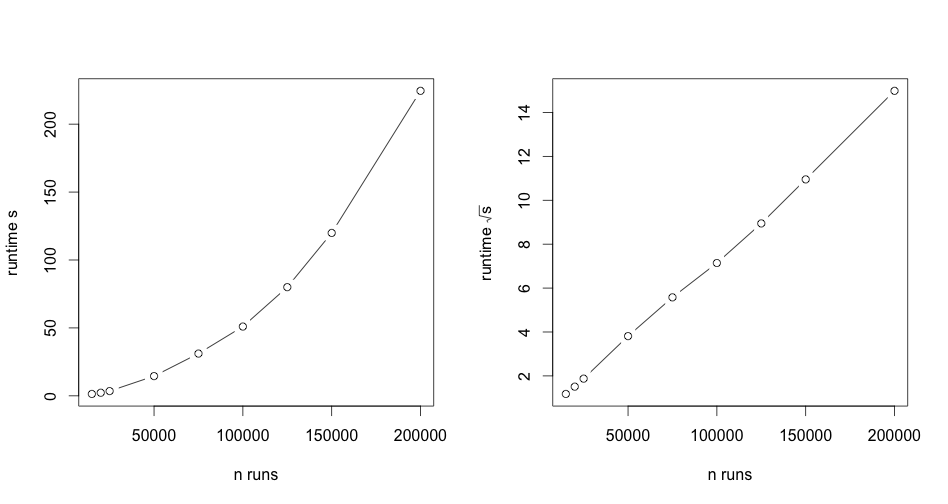
\includegraphics[width=\textwidth]{graph1.png}
\caption{\textit{Runtime values in seconds for a series of \textit{n}
  repetitions of the investigated algorithm. The left panel shows the
  measured times. For the right panel, the square root for each time
  value was calculated before plotting.}}
\label{fig:graph}
\end{figure}

The resulting runtime values, shown in the left of figure
\ref{fig:graph}, where transformed by calculating the square
root. The transformed data is shown in the right panel of figure 
\ref{fig:graph}. Then linear regression was calculated on the
transformed data (\textit{table\ref{tab:regression}}).

\begin{table}[]
\caption{\textit{Linear regression of the transformed experimental data}}
\label{tab:regression}
\begin{tabular}{lll}

gradient &  & $7.348 \times 10^{-5}$ \\
intercept &  & $1.393 \times 10^{-2}$ \\
$R^2$ &  & 0.9988 \\ 
\end{tabular}
\end{table}

The obtained linear equation was then transformed back to yield a
quadratic function as shown in equation (\ref{eq:quadratic}).

\begin{equation} \label{eq:quadratic}
y = 5.4 \times 10^{-9}x^2 + 2.1 \times 10^{-6}x + 0.2 \times 10^{-4}
\end{equation}

Then $c$ was determined according to equation (\ref{eq:limes}) and
$n_0$ was determined by solving the quadratic equation resulting from
$f(n) = g(n)$ (Table \ref{tab:ordo}, figure \ref{fig:ordo}). 



\begin{table}[]
\caption{\textit{Calculated value for ordo determination}}
\label{tab:ordo}
\begin{tabular}{lll}
$c$                       &  & $6.4 \times 10^{-9}$ \\
\multicolumn{1}{c}{$n_0$} &  & 2060                
\end{tabular}
\end{table}


\begin{figure} 
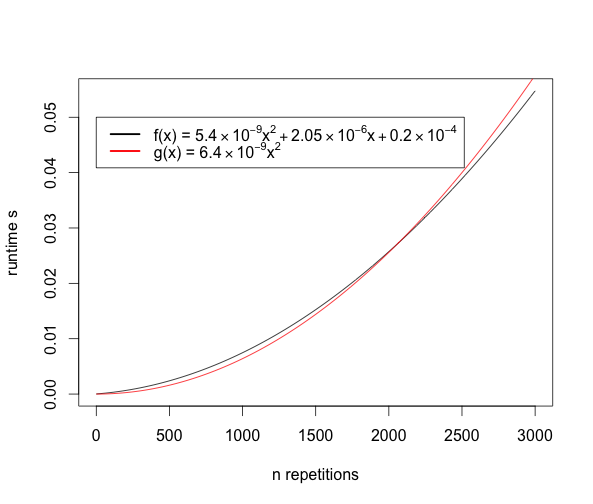
\includegraphics[width=\textwidth]{ordo.png}
\caption{\textit{Comparison of $f(x)$ and $O(g(x))$ in the range of $n_{0}$
  which was determined to be at about $n = 2600$.}}
\label{fig:ordo}
\end{figure}

\subsection{Asymptotic Complexity Analysis}
\subsubsection{Worst Case}

\begin{listing}\label{ls:worst}
\begin{verbatim}

1:  1 * [<-] + 
2:  1 * [<-] + 
3:  (numElements + 1) * 
    (3 * [get] + 1 * [<] +  1 * [=] + 1 * [AND]) + 
4:  numElements * (1 * [<-]) +
5:  init:
    (numElements * (numElements -1) / 2 + 1) *
    (1 * [get] + 1 * [-] + 1 * [<-]) +
 
    cond success + counter: 
    numElements * (numElements - 1) / 2) *
    (2 * [get] + 1 * [>] + 1 * [--]) +

    cond fail:
    numElements * 
    (2 * [get n] + 1 * [>]) +

6:  (numElements * (numElements - 1) / 2) * 
    (2 * [get] + 2 * [list[]] + 1 * [-] + 1 * [<] + 
7:      1 * [get] + 1 * [list[]] + 1 * [<-] +
8:      1 * [get] + 1 * [-] + 1 * [list[]] + 1 * [<-] + 
9:      2 * [get] + 1 * [-] + 1 * [ <-] +
10:     1 * [<-] ) +
11: numElements * (1 * [get] + 1 * [+] + 1 * [<-] +
12: 1 * return

set numElements = x

1:  1 + 
2:  1 + 
3:  (x + 1) * 6  
4:  x * 1
5:  (x * (x-1) / 2 + 1) * 3 +
    (x * (x - 1) / 2) * 4 +
    x * 3 +
6:  (x * (x - 1) / 2) * (6 +
7:    3 + 
8:    4 +
9:    4 + 
10:   1) + 
11: x * 3 +
12: 1 

Hence:
1 + 1 + 6x + 6 + x + 1.5x^2 - 1.5x + 3 + 2x^2 - 2x + 
3x + 9x^2 - 9x + 3x + 1

= 12.5x^2 + 4.5x + 12

\end{verbatim}
\caption{\textit{Determining the `worst case' complexity for the given
    `bubblesort' algorithm. The line numbers correspond to those in the listing (\ref{ls:bubble})}.}
\end{listing}

\subsubsection{Best case}

\begin{listing}\label{ls:best}
\begin{verbatim}
1:  1 * [<-] +
2:  1 * [<-] +
3:  2 * (3 * [get] + 1 *[<] + 1 * [and] + 1* [==]) +
4:  1 * [<-] +
5:  init:
    1 * [get] + 1 * [-] + 1 * [<-] +

    cond success + counter:
    (numElements - 1) * (1 * [get] + 1 * [>]) + 1 * [--]) +
    
    cond fail:
    1* [get] + 1 * [>] + 
6:  (numElements - 1) * 
    (2 * [get] +  2 * list[] + 1 * [-] + 1 * [<]) +
11: 1 * [get] + 1 * [+] + 1 * [<-]
12: 1 * [return]

set numElements = x

1:  1 +
2:  1 +
3:  2 * 6 +
4:  1 +
5:  3 + 
    (x - 1) * 3 +
    2 +
6:  (x - 1) * 6 +
11: 3 +
12: 1 

Hence:
1 + 1 + 12 + 1 + 3 + 3x - 3 + 2 + 6x -6 + 3 + 1
= 9x + 15

\end{verbatim}
\caption{Determining the `best case' complexity for the given
  `bubblesort' algorithm. The line numbers correspond to those in
  listing xxx}
\end{listing}

\begin{table}[]
\caption{\textit{Determination of $ordo$ for `Best' and `Worst Case'}}
\label{tab:ordo}
\begin{tabular}{llcc}
&  & Worst Case & Best Case \\ 
\hline
$f(n)$ &  & \multicolumn{1}{c}{$12.5n^2+4.5x+12$} & \multicolumn{1}{c}{$9x+15$} \\
$g(n)$ &  & \multicolumn{1}{c}{$13.5n^2$}         & \multicolumn{1}{c}{$10x$}   \\
$c$    &  & 13.5                                  & 10                          \\
$n_0$  &  & 7                                     & 15                          \\                         
\end{tabular}
\end{table}

show plot

\section{Discussion}
\subsection{Experimental Complexity Analysis}

\subsection{Asymptotic Complexity Analysis}
\subsubsection{Worst Case}
Line 1, 2 and 12 run just once. Line 3 runs \verb!numElements + 1! times. Lines
4 and 11 run \verb!numElements! times. Line 5 runs
\verb!(numElements * (numElements - 1)) / 2) + 1! 
times. The lines 6 to 10 run \verb!numElements * (numElements - 1) / 2! times. 
The \verb!downto! in \verb!for m <- (numElements - 1) downto n! was
interpreted as `larger than' condition.


\addcontentsline{toc}{section}{\refname}
\bibliography{references}

\end{document}
